\tikzset{every picture/.style={line width=0.75pt}} %set default line width to 0.75pt        

\newcommand\mergeleftpict{
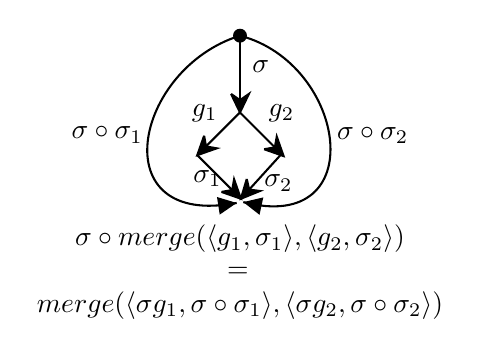
\begin{tikzpicture}[x=0.75pt,y=0.75pt,yscale=-1,xscale=1]
%\begin{tikzpicture}[x=0.75pt,y=0.75pt,yscale=-1,xscale=1, transform canvas={scale=0.6}]
%uncomment if require: \path (0,156);
%set diagram left start at 0, and has height of 156

\draw    (135,4) -- (135,41) ;
\draw [shift={(135,41)}, rotate = 270] [color={rgb, 255:red, 0; green, 0; blue, 0 }  ][fill={rgb, 255:red, 0; green, 0; blue, 0 }  ]  (8.93,-4.29) -- (0,0) -- (8.93,4.29) -- (5.93,0) -- (8.93,-4.29)    ;
\draw [shift={(135,4)}, rotate = 90] [fill={rgb, 255:red, 0; green, 0; blue, 0 }  ] [draw opacity=0]    (0, 0) circle [x radius= 3.35, y radius= 3.35]   ;
\draw    (135,41) -- (114.44,61.56) ;
\draw [shift={(114.44,61.56)}, rotate = 315] [color={rgb, 255:red, 0; green, 0; blue, 0 }  ][fill={rgb, 255:red, 0; green, 0; blue, 0 }  ]  (8.93,-4.29) -- (0,0) -- (8.93,4.29) -- (5.93,0) -- (8.93,-4.29)    ;

\draw    (135,41) -- (156,62) ;
\draw [shift={(156,62)}, rotate = 225] [color={rgb, 255:red, 0; green, 0; blue, 0 }  ][fill={rgb, 255:red, 0; green, 0; blue, 0 }  ]  (8.93,-4.29) -- (0,0) -- (8.93,4.29) -- (5.93,0) -- (8.93,-4.29)    ;

\draw    (114.44,61.56) -- (135.44,82.56) ;
\draw [shift={(135.44,82.56)}, rotate = 225] [color={rgb, 255:red, 0; green, 0; blue, 0 }  ][fill={rgb, 255:red, 0; green, 0; blue, 0 }  ]  (8.93,-4.29) -- (0,0) -- (8.93,4.29) -- (5.93,0) -- (8.93,-4.29)    ;

\draw    (155,61) -- (135.44,82.56) ;
\draw [shift={(135.44,82.56)}, rotate = 312.22] [color={rgb, 255:red, 0; green, 0; blue, 0 }  ][fill={rgb, 255:red, 0; green, 0; blue, 0 }  ]  (8.93,-4.29) -- (0,0) -- (8.93,4.29) -- (5.93,0) -- (8.93,-4.29)    ;

\draw    (133.4,84.6) .. controls (68.25,97) and (83.75,20) .. (135,4) ;

\draw [shift={(133.4,84.6)}, rotate = 171.16] [fill={rgb, 255:red, 0; green, 0; blue, 0 }  ] [draw opacity=0] (8.93,-4.29) -- (0,0) -- (8.93,4.29) -- (8.93,-4.29)    ;
\draw    (136.6,84.2) .. controls (198.6,100.2) and (186.75,17.5) .. (135,4) ;

\draw [shift={(136.6,84.2)}, rotate = 12.35] [fill={rgb, 255:red, 0; green, 0; blue, 0 }  ] [draw opacity=0] (8.93,-4.29) -- (0,0) -- (8.93,4.29) -- (8.93,-4.29)    ;

\draw (135,102) node   {$\sigma \circ merge( \langle g_{1} ,\sigma _{1} \rangle ,\langle g_{2} ,\sigma _{2} \rangle )$};
\draw (145,19) node   {$\sigma $};
\draw (118,41.5) node   {$g_{1}$};
\draw (155,41.5) node   {$g_{2}$};
\draw (119.33,73) node   {$\sigma _{1}$};
\draw (153.5,75) node   {$\sigma _{2}$};
\draw (71,51.8) node   {$\sigma \circ \sigma _{1}$};
\draw (199,52.2) node   {$\sigma \circ \sigma _{2}$};
\draw (135,134) node   {$merge( \langle \fillterm{\sigma}{g_{1}} ,\sigma \circ \sigma _{1} \rangle ,\langle \fillterm{\sigma}{g_{2}} ,\sigma \circ \sigma _{2} \rangle )$};
\draw (134,118) node   {$=$};

\end{tikzpicture}
}


\newcommand\mergerightpict{

 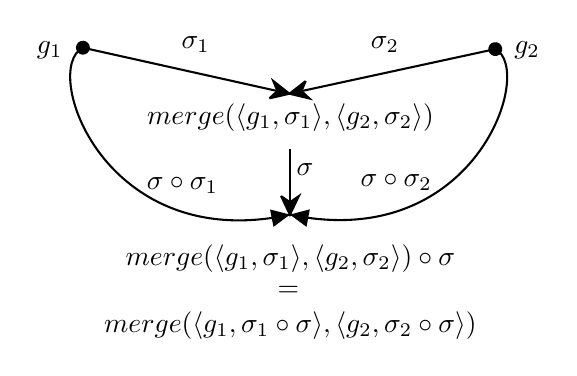
\begin{tikzpicture}[x=0.75pt,y=0.75pt,yscale=-1,xscale=1]
%\begin{tikzpicture}[x=0.75pt,y=0.75pt,yscale=-1,xscale=1, transform canvas={scale=0.6}]
%uncomment if require: \path (0,300); 
%set diagram left start at 0, and has height of 300

\draw    (130.75,110.75) .. controls (220.33,129.67) and (249,40.67) .. (229.67,31) ;

\draw [shift={(130.75,110.75)}, rotate = 10.75] [fill={rgb, 255:red, 0; green, 0; blue, 0 }  ] [draw opacity=0] (8.93,-4.29) -- (0,0) -- (8.93,4.29) -- (8.93,-4.29)    ;
\draw    (130.75,110.75) .. controls (41,130.33) and (10.42,40.42) .. (31,30.33) ;
\draw [shift={(31,30.33)}, rotate = 317.88] [fill={rgb, 255:red, 0; green, 0; blue, 0 }  ] [draw opacity=0]    (0, 0) circle [x radius= 3.35, y radius= 3.35]   ;
\draw [shift={(130.75,110.75)}, rotate = 168.87] [fill={rgb, 255:red, 0; green, 0; blue, 0 }  ] [draw opacity=0] (8.93,-4.29) -- (0,0) -- (8.93,4.29) -- (8.93,-4.29)    ;
\draw    (229.67,31) -- (130.5,52.5) ;
\draw [shift={(130.5,52.5)}, rotate = 347.77] [color={rgb, 255:red, 0; green, 0; blue, 0 }  ][fill={rgb, 255:red, 0; green, 0; blue, 0 }  ]  (8.93,-4.29) -- (0,0) -- (8.93,4.29) -- (5.93,0) -- (8.93,-4.29)    ;
\draw [shift={(229.67,31)}, rotate = 167.77] [fill={rgb, 255:red, 0; green, 0; blue, 0 }  ] [draw opacity=0]    (0, 0) circle [x radius= 3.35, y radius= 3.35]   ;
\draw    (31,30.33) -- (130.5,52.5) ;
\draw [shift={(130.5,52.5)}, rotate = 192.56] [color={rgb, 255:red, 0; green, 0; blue, 0 }  ][fill={rgb, 255:red, 0; green, 0; blue, 0 }  ]  (8.93,-4.29) -- (0,0) -- (8.93,4.29) -- (5.93,0) -- (8.93,-4.29)    ;

\draw    (130.75,79.28) -- (130.75,110.75) ;
\draw [shift={(130.75,110.75)}, rotate = 270] [color={rgb, 255:red, 0; green, 0; blue, 0 }  ][fill={rgb, 255:red, 0; green, 0; blue, 0 }  ]  (8.93,-4.29) -- (0,0) -- (8.93,4.29) -- (5.93,0) -- (8.93,-4.29)    ;


\draw (131,132) node   {$merge( \langle g_{1} ,\sigma _{1} \rangle ,\langle g_{2} ,\sigma _{2} \rangle ) \circ \sigma $};
\draw (130,148) node   {$=$};
\draw (131,164) node   {$merge( \langle g_{1} ,\sigma _{1} \circ \sigma \rangle ,\langle g_{2} ,\sigma _{2} \circ \sigma \rangle )$};
\draw (131,64) node   {$merge( \langle g_{1} ,\sigma _{1} \rangle ,\langle g_{2} ,\sigma _{2} \rangle )$};
\draw (245,31.5) node   {$g_{2}$};
\draw (15,31.5) node   {$g_{1}$};
\draw (138,89) node   {$\sigma $};
\draw (85.33,29) node   {$\sigma _{1}$};
\draw (176.5,29) node   {$\sigma _{2}$};
\draw (79,96.8) node   {$\sigma \circ \sigma _{1}$};
\draw (182,95.2) node   {$\sigma \circ \sigma _{2}$};


\end{tikzpicture}
}